\documentclass[a4paper, 12pt]{article}

%\usepackage{savetrees}
\usepackage{graphicx}

\title {Student Robotics 2010\\ Rulebook}
\date{\today}
\setcounter{tocdepth}{1}


\begin {document}

\maketitle

\noindent The following defines the rules and regulations of the Student Robotics 2010 competition.

\newcounter{rule}[section]
\newcommand{\rcn}{\stepcounter{rule}\arabic{section}.\arabic{rule}}
\renewcommand{\labelenumi}{\rcn}

\section {Game Rules}
\label{game-rules}

\begin{enumerate}
\item There will be a maximum of 4 robots in a match.
\item A match lasts 180 seconds.
\item Matches are started and stopped by the Student Robotics radio system\footnote{The Student Robotics radio system is supplied as part of the kit.
 It is part of the power board, and is used for safety cut-off, start-match and stop-match signals.}.
\item There is one type of game that will be played, it is called \textbf{QuackMan}.

At the start of a match, the arena will be populated with 46 tokens.
The tokens are laid out in a pattern of one on the vertex of each square metre in the arena, except for where the three spots where this is too close to the central tower where there are no tokens.
At the top of the tower there is a rubber duck.

\item Robots must start the match within their team's zone.
 Robots will be handed to a [[BLUE SHIRT]] who will place the robot in the appropriate start zone before the beginning of the match.

\item At the end of a match, after all tokens have settled, a team's ``\textbf{game points}'' will be counted.
 These are used to rank teams before competition league points are awarded.

\item Game points are awarded as follows:
\begin{itemize}
\item Red tokens collected are worth 1 game point.
\item Blue tokens collected are worth -5 game points.
\item The duck is worth 100 game points.
\end{itemize}

\item At the end of a game, the team with the \emph{most} game points is awarded 4 points towards the competition league.
 The team with the second most is awarded 3.
 The team with the third most is awarded 2 points, and the team with the fewest game points is awarded 1 point.
 Teams whose robot was not entered into the round, or who were disqualified from the round, will be awarded no points.

\end{enumerate}

\newpage
\section {Regulations}
\label{regs}

\begin{enumerate}
\item Robots must fit within a cube with 500mm sides.
\item Robots must have a switch which enables/disables the power to the motors.  This switch must be accessible from the outside of the robot.
\item No remote control systems may be used, with the exception of the Student Robotics radio system for starting and stopping matches.
\item This is a non-contact sport (accidental bumps and scrapes are inevitable).
\item Robots should not intentionally damage tokens, zones or arena.
\item Student Robotics reserves the right to look at your robot software and hardware at any time.
\item All kit deployed by Student Robotics remains the property of Student Robotics.
\item The Judge's decision is final.
\end{enumerate}

\newpage
\section{Specifications}
\newcounter{rulei}[subsection]
\newcommand{\rcnii}{\stepcounter{rulei}\arabic{section}.\arabic{subsection}.\arabic{rulei}}
\renewcommand{\labelenumi}{\rcnii}

\subsection{Arena}
\begin{enumerate}
\item The match arena floor is an 8m x 8m square.  The tolerance of the two arena dimensions is $\pm0.25m$.
\item The floor of the arena is made of white plastic coated hardboard.  White Gaffer tape will be in place over the joints between hardboard sheets.
\item The arena walls are $600\pm30mm$ high and are made of the same material as the arena floor.
\item The arena is encased in a scaffolding structure, which is approximately $3m$ tall (revised measurements will be provided within a week of the Kick Start event).  The scaffolding structure is covered in netting in order to prevent balls from escaping from the arena.
\end{enumerate}

\subsection{Balls}
\label{balls}
\begin {enumerate} 
\item Balls have a radius of 55mm, and can be purchased from Argos with the part number 366/5514.  Each team's kit contains a small number of these.
\item The following ball colours will be used: red, blue, yellow and green.
\end {enumerate}

\subsection{Zones}
\begin {enumerate}
\item The arena contains 4 zones.  Each zone occupies one quarter of the arena and has an associated colour and net.  Figure~\ref{fig:arena} shows the dimensions and colours of the zones.
\item The zone is bounded by a border of black Gaffer tape stuck to the arena floor.  Each arm of the Gaffer tape cross has a different width.  The four widths are 50, 75, 100 and 125mm.
\end {enumerate}

\begin{figure}
\begin{center}
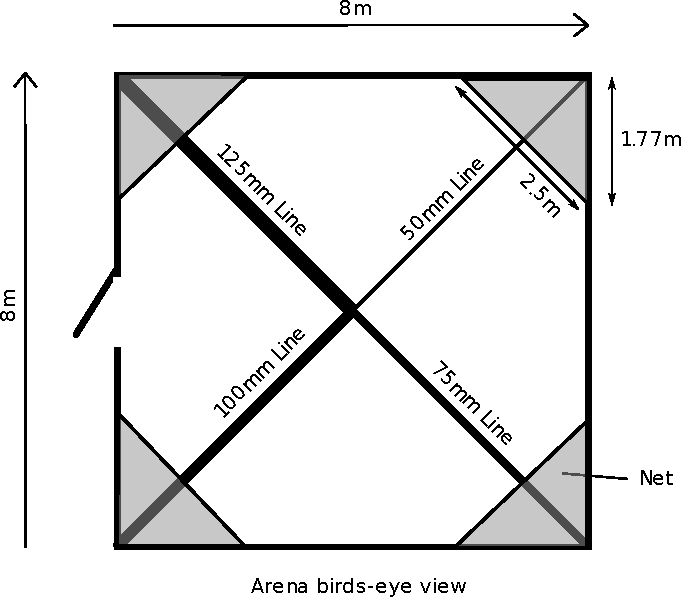
\includegraphics[keepaspectratio, width=\textwidth]{./images/arenadim.pdf}
\caption{\label{fig:arena}Arena dimensions and markings.}
\end{center}
\end{figure}

\begin{figure}
\begin{center}
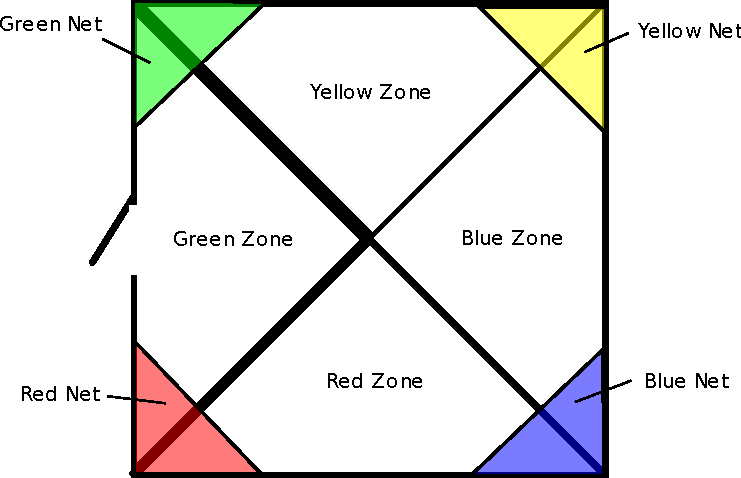
\includegraphics[keepaspectratio, scale =1]{./images/colours.pdf}
\caption{\label{fig:zone}Zone and net colours.}
\end{center}
\end{figure}

\subsection{Nets}
\begin{enumerate}
\item The arena contains 4 nets.  Each net is a horizontal triangle of netting, held up by a diagonal rod of scaffold. Figure~\ref{fig:nets} shows the dimensions and positioning of the nets.
\item Square sections of the arena wall are coloured at their intersection below the nets, as shown in figure~\ref{fig:nets}.
\end{enumerate}

\begin{figure}
\begin{center}
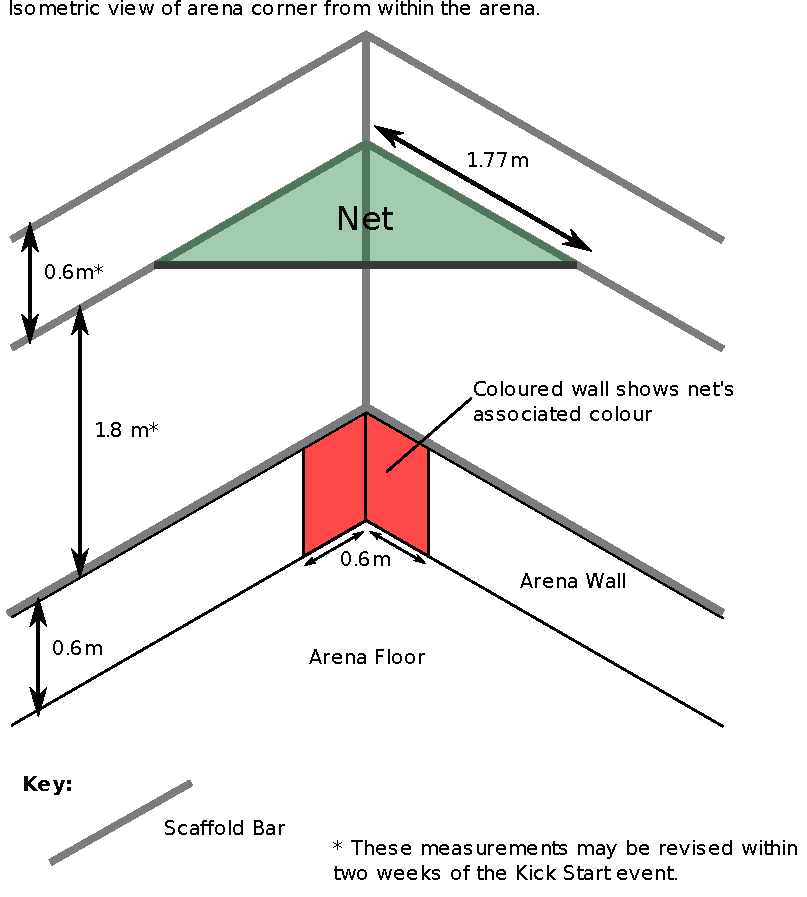
\includegraphics[keepaspectratio, scale =1]{./images/net.pdf}
\caption{\label{fig:nets}Zone and net colours.}
\end{center}
\end{figure}

\subsection{Robot Flags}
\label{sec:flags}
All robots must have a flagpole so that two flags can be mounted upon it:
\begin{description}
\item[Team Flag] The team flag is to be designed and created by the team.  It is optional and recommended.  The team flag allows the robot to be easily identified.  This flag must be mounted between 700mm and 900mm off the ground.  It must not extend more than 200mm from the flagpole.

The team flag must not sag below 700mm above the ground.
\item[Match Flag] The match flag is to be supplied by Student Robotics at the start of every match.  The match flag will slot over the top 100mm of the flagpole.  The top 100mm of the flagpole must have an external diameter of $5\pm1$mm so that the match flag can slot over it.  The match flags have an end-cap so that they will not slide down the flagpole.
\end{description}

The flagpole must be removable so that the robot can be placed within a box to check the size limit.  A diagram of the flagpole arrangement can be found in figure~\ref{fig:flag}.

\begin{figure}
\begin{center}
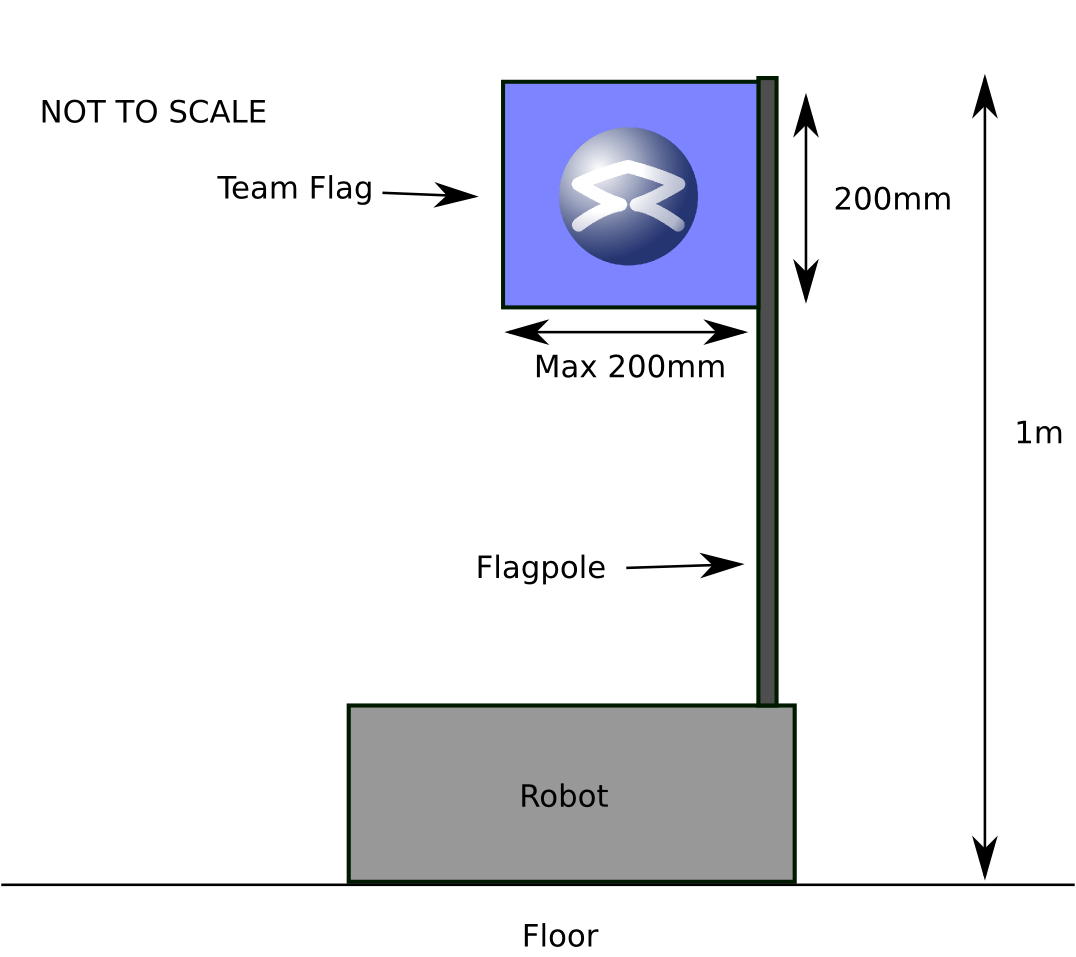
\includegraphics[keepaspectratio, scale =1]{./images/flag.png}
\caption{\label{fig:flag}Flagpole Dimensions}
\end{center}
\end{figure}
\clearpage

\section{Change log}
The following changes have been made to the rules since their initial release:
\begin{description}
\item [2010/03/20] Figure \ref{fig:ramp-dim} was changed to a more accurate image, with more sizes on it.
 Change the width of the gaffer tape in Rule 3.2.1 to $60mm$ to match the diagram.
\item [2009/10/06] Rule 2.10 was changed from ``Robots must have a flagpole attached'' to ``Robots \emph{may} have a flagpole attached''.
\end{description}

\end {document}
